%  \documentclass[DIV=12, a4]{scrartcl}
% \documentclass[10pt, a5paper]{scrartcl}
\documentclass[a4]{scrreprt}

\usepackage[
fancytheorems, 
fancyproofs,
noindent, 
%spacingfix, 
]{adam}



% \usepackage[margin=0.75in]{geometry}

\usepackage{tikz}

% \setcounter{section}{-1}

\title{Groups}
% \subtitle{Adam Kelly}
\author{Adam Kelly}
\date{Updated \today}

\begin{document}

\maketitle

\begin{abstract}
	This set of notes is a work-in-progress account of the course `Groups', originally lectured by Dr. Ana Khukhro in Michaelmas 2020 at Cambridge. These notes are not a transcription of the lectures, but they do roughly follow what was lectured (in content and in structure).

	These notes are my own view of what was taught, and should be somewhat of a superset of what was actually taught. I frequently provide different explanations, proofs, examples, and so on in areas where I feel they are helpful. Because of this, this work is likely to contain errors, which you may assume are my own. If you spot any or have any other feedback, I can be contacted at \href{mailto:ak2316@cam.ac.uk}{ak2316@cam.ac.uk}.
\end{abstract}

\tableofcontents

\clearpage


\chapter{Groups}

`Groups' is a course which introduces you to the subject of \emph{Abstract Algebra}.
Indeed, while groups are one of the simplest and most basic of all the algebraic structures\footnote{Apart from `magmas' I suppose, but they don't tend to be a particularly useful notion.}, they are immensely useful and appear in almost every area of mathematics. 

\section{Definition of a Group}

We will begin our study of the subject by defining formally what a group is.

\begin{definition}[Group]
	A \vocab{group} is a set $G$ with a binary operation\footnote{Some texts include an additional \emph{closure} axiom, but this is implied by $*$ being a binary operation on $G$.} $*$ which satisfies the axioms:
	\begin{itemize}
		\item \emph{Identity}. There is an element $e \in G$ such that $g * e = e * g = g$ for every $g \in G$.
		\item \emph{Inverses}. For every element $g \in G$, there is an element $g^{-1} \in G$ such that $g * g^{-1} = g^{-1} * g = e$.
		\item \emph{Associativity}. The operation $*$ is associative.
	\end{itemize}
\end{definition}

We typically refer to a group as defined above by $(G, *)$, which explicitly states that $*$ is the group operation. When the operation being used is clear, we can refer to the group by just $G$. We will also be omitting the group's operation symbol quite often, for example writing $gh = g * h$. 

 In a later section, we will look at some non-trivial examples of groups.

\subsection{Elementary Properties of Groups}

With the notion of a group now defined, we can now consider some basic facts that follow directly from the definition of a group. We will first address whether it is possible for a group to have multiple identity elements, or for an element to have multiple inverses (no).

\begin{proposition}[Uniqueness of the Identity and Inverse]
	Let $(G, *)$ be a group. Then there is a unique identity element, and for every $g \in G$, $g^{-1}$ is unique.
\end{proposition}
\begin{proof}
	To prove that the identity element is unique, let $e$ and $e'$ be identity elements of $G$. Then $e* e' = e$ and $e* e' = e'$ by definition, giving $e = e'$. 
	
	To prove that the inverses are unique, suppose that for some $g, h, k \in G$ we have $g* h = g *k = e$. Then $g^{-1}* g *h = g^{-1} *g * k$, implying $h = k$. The case of $h * g = k * g = e$ follows analogously.
\end{proof}

The next useful fact is the \emph{cancellation law}, whose proof bears a large resemblance to the proof that inverses are unique.

\begin{proposition}[Cancellation Law]
	If $(G, *)$ is a group, and $a, b, c \in G$, then $a*b = a*c$ and $b*a = c*a$ both imply $b = c$.
\end{proposition}
\begin{proof}
	Taking $a * b = a * c$ and left-multiplying by $a^{-1}$ we have $a^{-1} * a * b = a^{-1} * a * c$, that is, $b = c$. The other case follows analogously.
\end{proof}

The last proposition we will prove in this section gives us a useful result about computing inverses.

\begin{proposition}[Computing Inverses]
	Let $(G, *)$ be a group, and let $g, h \in G$. Then the following hold:
	\begin{enumerate}[label=(\roman*)]
		\item $(g*h)^{-1} = h^{-1} * g^{-1}$.
		\item $(g^{-1})^{-1} = g$.
	\end{enumerate}
\end{proposition}
\begin{proof}$ $\phantom{\qedhere}
	\begin{enumerate}[label=(\roman*)]
		\item We have $(g*h) * (h^{-1} * g^{-1}) =  g * (h * h^{-1}) * g^{-1} = g * g^{-1} = e$, so $(g*h)^{-1} = h^{-1} * g^{-1}$.
		\item Similarly, $g^{-1} * g = e$, so $(g^{-1})^{-1} = g$. \hfill \qedsymbol
	\end{enumerate}
\end{proof}

\subsection{Examples of Groups}

It's probably of some use to have concrete examples of groups in your head, so you can get a feel for what they are. In this section we will present some non-trivial examples of groups (and some examples of non-groups).

It should be recognized that commutativity is \emph{not} a group axiom, and the majority of groups are not commutative. We do have a name for groups where the binary operation is commutative though.

\begin{definition}[Abelian Groups]
	We say a group $(G, *)$ is \vocab{abelian} if $*$ is commutative, that is, if for any $g, h \in G$, $g * h = h * g$.
\end{definition}

In this section, we will consider examples of both abelian and non-abelian groups\footnote{If you are not familiar with some of the concepts used, such as matrices or modular arithmetic, feel free to ignore those examples.}. In the first few cases, the reasons why they are a group are stated. For the others, you should consider how they satisfy the group axioms yourself. 

\begin{example}[The Trivial Group]
	The \vocab{trivial group} is a group whose only element is the identity, $\{ e \}$.
\end{example}

\begin{example}[Additive Group of Integers]
	$(\Z, +)$ is an group. We have
	\begin{itemize}
		\item The identity element $0 \in Z$, as $a + 0 = 0 + a = a$ for any $a \in \Z$
		\item The inverse of $a \in \Z$ being $-a$, as $a + (-a) = (-a) + a = 0$. 
		\item The operation $+$ is associative and commutative.
	\end{itemize}
\end{example}
We also have the additive group of rationals $(\Q, +)$, of reals $(\R, +)$, and of complex numbers $(\C, +)$ for the same reasons.

\begin{example}[Addition Modulo $n$]
	Let $n \in \N$, and let $\Z/n \Z = \{0, 1, \dots, n - 1\}$ denote the set of residues modulo $n$. Then $(\Z/n\Z, +)$ is a group (where addition is done modulo $n$). We have
	\begin{itemize}
		\item The identity element is $0 \pmod{n}$, as $a + 0 \equiv 0 + a \equiv a \pmod{n}$.
		\item The inverse of $a \in \Z/n\Z$ is $-a$, as $a + (-a) \equiv 0 \pmod{n}$.
		\item Addition modulo $n$ is associative.
	\end{itemize}
\end{example}

\begin{example}[Non-Zero Rationals]
	Let $\Q^\times$ denote the set of non-zero rationals. Then $(\Q^\times, \times)$ is a group.
\end{example}
Similarly, we also have the groups $(\R^\times, \times)$ and $(\C^\times, \times)$.

\begin{example}[Multiplication Modulo $p$]
	Let $p$ be a prime, and let $(\Z / p \Z)^\times$ denote the set of non-zero residues modulo $p$. Then $((\Z / p \Z)^\times, \times)$ is a group (where multiplication is done modulo $p$).
\end{example}

\begin{example}[General Linear Group]
	Let $\GL_n(\R)$ be the set of $n \times n$ matrices with non-zero determinant. Then $(\GL_n(\R), \times)$ is the \vocab{general linear group}\footnote{Using matrix multiplication}.
\end{example}

\begin{example}[Special Linear Group]
	Let $\SL_n(\R)$ be the set of $n \times n$ matrices with determinant 1. Then $(\SL_n(\R), \times)$ is the \vocab{special linear group}.
\end{example}

\subsection*{Non-Examples of Groups}

We will now give some examples of sets with operations that are not groups. It should be useful to think about why each example does not satisfy the group axioms.

\begin{example}[Non-Examples of Groups]
	The following are are all \emph{not} groups.
	\begin{itemize}
		\item $(\Z, \times)$
		\item $(\Q, \times)$
		\item The set of $2\times 2$ matrices with matrix multiplication.
		\item $(\R, *)$ where $r  * s = r\times r \times s$
		\item $(\N, *)$ where $n * m = |n - m|$.
	\end{itemize}
\end{example}

\section{Subgroups}

Given any mathematical structure, it can be useful to know about its \emph{substructure}. In the case of a group $(G, *)$, one might ask the question is there some subset $H \subseteq G$ that still acts like a group? This motivates the introduction of \emph{subgroups}.

\begin{definition}[Subgroups]
	Let $(G, *)$ be a group. A subset $H \subseteq G$ is a \vocab{subgroup} of $G$ if $(H, *)$ is also a group. If $H$ is a subgroup of $G$, we will write $H \leq G$.
\end{definition}

\begin{example}[Examples of Subgroups]
	The following are subgroups.
	\begin{itemize}
		\item For any group $G$, we have the \vocab{trivial subgroups} $\{ e \} \leq G$ and $G \leq G$.
		\item $\Z \leq \Q \leq \R \leq \C$ with addition.
		\item $\{ 0, 2, 4, \dots \} \leq \Z$ with addition.
		\item $\SL_n(\R) \leq \GL_n(\R)$ with matrix multiplication.
	\end{itemize}
\end{example}


Checking whether something is a subgroup is easier than checking if something is a group, since we already know about the structure of the group. To check whether $H$ is a subgroup of $(G, *)$, we can just check the following hold:
\begin{itemize}
	\item \emph{Closure}. $*$ is closed in $H$.
	\item \emph{Identity}. $e \in H$.
	\item \emph{Inverses}. For $h \in H$, we also have $h^{-1} \in H$. 
\end{itemize}

These can all be combined into a single test, that is sometimes known as the `subgroup checking lemma'.

\begin{lemma}[Subgroup Criterion]
	A subset $H$ of a set $G$ is a subgroup of $(G, *)$ if and only if $H$ is non-empty and $x * y^{-1} \in H$ for all $x, y \in H$.
\end{lemma}
\begin{proof}[Proof Sketch]
	First check that the conditions of $H$ being non-empty and $x * y^{-1} \in H$ imply that it's a subgroup. Then, show that if $H$ is not a subgroup, then either $H$ is empty or $x * y^{-1} \not\in H$ for some $x, y \in H$.
\end{proof}

As an example of using subgroups, let's try to characterize all of the subgroups of $(\Z, +)$.

\begin{theorem}[Subgroups of $\Z$]\label{thm:subgroups-of-z}
	The subgroups of $(\Z, +)$ are precisely the subsets of the form $n \Z$ for $n \in N$, where $n\Z = \{n k \; : \; k \in \Z\}$.
\end{theorem}
\begin{proof}
	First, we prove that $n \Z$ is a subgroup. Fix $n \in \N$.
	\begin{itemize}
		\item \emph{Closure}. Given $n k_{1}, n k_{2} \in n \Z,$ then $n k_{1}+n k_{2}=n\left(k_{1}+k_{2}\right) \in n \Z$.
		\item \emph{Identity}. $0 =n \cdot 0 \in n \Z$.
		\item \emph{Inverses}. The inverse of $n k$ is $-n k=n(-k) \in n \Z$.
	\end{itemize}
Thus each is subgroup. Now we prove that there is no other subgroups.

Let $H \leq Z$. If $H=\{0\}$, then $H \equiv 0 \Z$. If not, then take the smallest positive element in $H$ (namely $n$ ). since $H$ is a subgroup, it's closed and contains inverses, so $n+n+\cdots+n \in$ $H$ and $-n-n-n-\cdots-n \in H,$ so $n \Z \subseteq H$.

Suppose, for a contradiction, there is some $k \in H$ such that $k \neq n \Z .$ So, there is some integer $n$ such that $n m<k<n(m+1) .$ But then $0 \leq k-n m<n,$ and $k-n m \in H$ which is a contradiction, so $H=n \Z$.
\end{proof}

We can use the definition of a subgroup to prove some elementary facts.
\begin{proposition}[Elementary Properties of Subgroups]
	Let $G$ be a group.
	\begin{enumerate}[label=(\roman*)]
		\item Let $H$ and $K$ be subgroups of $G$. Then $H \cap K \leq G$.
		\item If $K \leq H$ and $H \leq G$ then $K \leq G$ (being a subgroup is transitive).
		\item If $K \subset H$, $H \leq G$ and $K \leq G$, then $K \leq H$. 
	\end{enumerate}
\end{proposition}
\begin{proof} There is multiple ways to prove these, but we will use the subgroup criterion as an example of it being used.\phantom{\qedhere}
	\begin{enumerate}[label=(\roman*)]
		\item Note that $H \cap K$ is not empty as $e \in H$ and $e \in K$. Then, for any $x, y \in H \cap K$, it suffices to show that $x * y^{-1} \in H$. By the subgroup criterion, we have $x * y^{-1} \in H$ and $x*y^{-1} \in K$, thus $x * y^{-1} \in H \cap K$, and we are done.
		\item If $K \leq H$, then for any $x, y \in K$, we have $x * y^{-1} \in K$. Then as $K \subset H \subset G$, we must have $x * y^{-1} \in G$, and thus $K \leq H$.
		\item As $K \leq G$, we know $K$ is non-empty. Thus it suffices to show that $x * y^{-1} \in K$ for any $x, y \in H$. But this is implied by $K \leq G$ and the subgroup criterion, and thus as $K \subset H$, $K \leq H$. \hfill \qedsymbol
	\end{enumerate}
\end{proof}

\subsection{Generators}

We will now consider a certain kind of subgroup, which is specified by some of the elements it contains.

\begin{definition}[Subgroup Generated By A Subset]
	For some set $X \subseteq G$, we define the \vocab{subgroup generated by $X$}, $\langle X \rangle$, to be the smallest subgroup of $G$ which contains $X$.
\end{definition}

From this definition, we can see that we must have $e \in \langle X \rangle$ and $X \subseteq \langle X\rangle$. Also, $\langle X \rangle$ must contain all products of elements in $X$ and their inverses.
We can put this in a more useful form with the following proposition.

\begin{proposition}
	Let $X$ be a non-empty subset of $G$. Then $\langle X \rangle$ is the set of elements of $G$ of the form 
	$x_1^{\alpha_1} x_2^{\alpha_2} \cdots x_k^{\alpha_k}$ where $x_i \in X$ (not necessarily distinct), $\alpha_i = \pm 1$ and $k \geq 0$
	(For $k = 0$, we say the element is $e$).
\end{proposition}
\begin{proof}
	Let $T$ be the set of such elements. Clearly $T \subseteq \langle X \rangle$, and also clearly $T$ is a subgroup of $G$. We also have that $X \subseteq T$ so $\langle X \rangle \subseteq T$. Thus $T = \langle X \rangle$.
\end{proof}
  
\begin{example}
	We have $(\Z, +) = \langle 1 \rangle = \langle 2, 3 \rangle$\footnote{Note that we write $\langle 2, 3\rangle$ instead of $\langle \{2, 3\} \rangle$.}, and $\Z/5\Z = \langle 1 \rangle = \langle 3 \rangle$.
\end{example}

In the above examples, we found that there was some subset of the elements in each of the group where if we considered the subgroup generated by those elements, we get the entire group.
There is a special name for such subsets.

\begin{definition}[Generators]\label{def:generator}
	If $X$ is a subset of $G$ such that $\langle X \rangle = G$, then we call $X$ a \vocab{generating set} of $G$.
\end{definition}

Notably, these generators are not necessarily unique, as can be seen in the example above.


\section{Homomorphisms}

Imagine you had two groups, $G$ and $H$ and you wanted to think of a function from $H$ to $G$ that preserved some of the structure of the group.
Let's say the function was $\phi : H \rightarrow G$. We could take any two elements $h_1, h_2 \in H$, and we could find $h_1 h_2$, and then apply $\phi$ to get $\phi(h_1 h_2)$.
Alternatively, we could try and find $\phi(h_1)$ and $\phi(h_2)$, and then get $\phi(h_1) \phi(h_2)$. If these were the same, then the function $\phi$ would indeed preserve some of the structure of the group. This motivates the introduction of \emph{homomorphisms}.

\begin{definition}[Homomorphism]
	Let $(G, *_G)$ and $(H, *_H)$ be groups. A function $\phi : H \rightarrow G$ is a \vocab{group homomorphism} if for all $a, b \in H$,
	$$
	\phi(a *_H b) = \phi(a) *_G \phi(b).
	$$
\end{definition}

\begin{example}[Inclusion Function]
	If $H \leq G$, then the function $\iota : H \rightarrow G$ that has $\iota(h) = h$ for $h \in H$ is a homomorphism. It is also injective.
\end{example}

\begin{example}
	The function $\phi : \Z\rightarrow \Z/n\Z$ with $\phi(k) = k \pmod{n}$ is a homomorphism, since for $k, l \in \Z$,
	$$
\phi(k + l) = (k + l) \bmod{n} = (k \bmod{n}) + (l \bmod{n}) = \phi(k) + \phi(l).
	$$
	$\phi$ is also surjective, since $\{0, 1, \cdots, n - 1\}$ are all the possible residues modulo $n$.
\end{example}

\begin{example}
	The function $\phi : (\R, + )\rightarrow (\R^*, \cdot)$ where $x \rightarrow e^x$ is a homomorphism. We have
	$$
	\phi(x + y) = e^{x + y} = e^x \cdot e^y = \phi(x) \cdot \phi(y).
	$$
	It is injective, as $e^x = e^y$ implies $x = y$ using logarithms, and surjective, as given $a \in \R^*$, $\phi(\log a) = e^{\log a} = a$.
\end{example}

We can see some natural consequences of this definition of a homomorphism, which shows how well it preserves the group's structure.

\begin{proposition}[Properties of Homomorphisms]
	Let $\phi : H \rightarrow G$ be a homomorphism.
	\begin{enumerate}[label=(\roman*)]
		\item $\phi(e_h) = e_g$. 
		\item $\phi(h^{-1}) = \phi(h)^{-1}$ for all $h \in H$.
		\item If $\psi : G \rightarrow K$ is another homomorphism, then $\psi \circ \phi : H \rightarrow K$ is also a homomorphism.
	\end{enumerate}
\end{proposition}
\begin{proof}
	$ $ \phantom{\qedhere}
	\begin{enumerate}[label=(\roman*)]
		\item We have $e_H *_H e_H = e_H$, so $\phi(e_H * e_H) = \phi(e_H) *_G \phi(e_H) = \phi(e_H)$, so by the cancellation law, $\phi(e_H) = e_G$.
		\item Consider $\phi(h) *_G \phi(h^{-1}) = \phi(h *_H h^{-1}) = \phi(e_H) = e_G$, by (i). So $\phi(h) *_G = \phi(h^{-1}) = e_G$ which is the defining property of an inverse, so $\phi(h^{-1}) = \phi(h)^{-1}$.
		\item We have 
		\begin{align*}
			(\psi \circ \phi)(a *_H) &= \psi(\phi(a *_H b))\\
									 &= \psi(\phi(a) *_G \phi(b))\\ 
									 &= \psi(\phi(a)) *_K \psi(\phi(b)) \\
									 &= (\psi \circ \phi)(a) *_K (\psi \circ \phi)(b),
		\end{align*}
		so $\psi \circ \phi$ is a homomorphism from $H \rightarrow K$.\hfill \qedsymbol
	\end{enumerate}
\end{proof}


There is a special case of homomorphism, which we can use to define when two groups `are the same'.

\begin{definition}[Isomorphism]
	If a function $\phi : H \rightarrow G$ is bijection, and $\phi$ is also a homomorphism from $H \rightarrow G$, then we say it is an \vocab{isomorphism}. We say two groups $H, G$ are \vocab{isomorphic}, written $H \cong H$ if there is an isomorphism from $H \rightarrow G$.
\end{definition}

Having an isomorphism between two groups can be thought of in a few ways. Because we have a bijection function between the two groups, the groups must have the same order. But also, because a homomorphism preserves the structure of the group, we must also have the same group-structure within each group. Thus, when we have two isomorphic groups, we can think of them as two different descriptions of the same group.

For example, we might claim that `there is exactly one group of order 2', and what we mean is that for any group of order 2, we can find an isomorphism to any other group of order 2. 

\begin{example}
	Consider the group $G = \{ 1, i, -1, -i \}$ with complex multiplication. Then $G \cong \Z / 4 \Z$. This is isomorphic with the isomorphism $\phi : G \rightarrow \Z / 4 \Z$, where
	\begin{align*}
		\phi(1) &= 0, \\
		\phi(i) &= 1, \\
		\phi(-1) &= 2, \\
		\phi(-i) &= 3
	\end{align*}
	The general case is true too, where the group $H = \{  e^{2 \pi i k/n} : 0 \leq k \leq n - 1 \}$ with complex multiplication is isomorphic to $\Z /n \Z$.
\end{example}

\begin{example}[$\Z$'s subgroups are isomorphic]
	$\Z \cong n \Z$ for $n \in \Z$, as defined in \autoref{thm:subgroups-of-z}. 
\end{example}

It's worth noting that because isomorphisms are bijective, we have the following result.

\begin{proposition}[Inverses of isomorphisms are isomorphisms]
	Let $\phi : H \rightarrow G$ be an isomorphism. Then $\phi^{-1} : G \rightarrow H$ is also an isomorphism.
\end{proposition}
\begin{proof}[Proof Sketch]
	Check that $\phi^{-1}$ is a homomorphism.
\end{proof}

\subsection{Kernels}

When dealing with homomorphisms, say $\phi : H \rightarrow G$, it is useful to be able to think about what elements in $H$ our homomorphism `reaches'.
Another useful idea is thinking about what elements in $H$ get mapped to the identity of $G$. To think about these questions, we use concepts of a homomorphism's \emph{image} and \emph{kernel}. 

\begin{definition}[Image]
	Let $\phi :H \rightarrow G$ be a homomorphism. We define the \vocab{image} of $\phi$ to be the set
	$$
	\image(\phi) = \{ g \in G \; : \; g = \phi(h) \text{ for some } h \in H  \}.
	$$
\end{definition}
\begin{definition}[Kernel]
	Let $\phi : H \rightarrow G$ be a homomorphism. We define the \vocab{kernel} of $\phi$ to be the set
	$$
	\kernel(\phi) = \{ h \in H \; : \; \phi(h) = e_G \}.
	$$
\end{definition}

Indeed, while both of these are subsets of $G$ and $G$ respectively, they are also subgroups.

\begin{proposition}[The Image and Kernel are Subgroups]
	Let $H$ and $G$ be groups and let $\phi : H \rightarrow G$ be a homomorphism. Then $\image(\phi)$ is a subgroup of $G$, and $\kernel(\phi)$ is a subgroup of $H$.
\end{proposition}
\begin{proof}
	We consider the two sets separately.
	\begin{enumerate}
		\item We will show $\image(\phi) \leq G$. For any $x, y \in \image(\phi),$ let $x = \phi(x')$ and $y = \phi(y')$ for $x', y' \in H$. Then
		$$
		\phi(x' {y'}^{-1}) = \phi(x')\phi(y')^{-1} = x y^{-1} \in \image(\phi),
		$$
		thus by the subgroup criterion $\image(\phi) \leq G$.
		\item Now we show $\kernel(\phi) \leq H$. For $x, y \in \kernel(\phi)$, we have $xy^{-1} \in \kernel(\phi)$, as 
		$$
		\phi(xy^{-1}) = \phi(x)\phi(y^{-1}) = \phi(x)\phi(y)^{-1} = e_G,
		$$
		so again using the subgroup criterion, $\kernel(\phi) \leq H$. 
	\end{enumerate}
\end{proof}

\begin{example}
	$\phi : \Z \rightarrow \Z/n\Z$, where $\phi(k) = k \pmod{n}$ has $\image(\phi) = \Z/n\Z$ and $\kernel(\phi) = n\Z$.
\end{example}

One of the beauties of introducing the kernel and image is that it allows us to easily see whether a homomorphism is surjective or injective.

\begin{proposition}[Surjectivity and Injectivity Criterion]
	Let $\phi : H \rightarrow G$ be a homomorphism.
	\begin{enumerate}[label=(\roman*)]
		\item $\phi$ is surjective iff $\image(\phi) = G$.
		\item $\phi$ is injective iff $\kernel(\phi) = \{e\}$.
	\end{enumerate}	
\end{proposition}
\begin{proof}
	The first is true by definition, so we prove (ii). Suppose $\phi$ is injective, then as we have $\phi(e_H) = e_G$, so $e_H$ must be the only element sent to $e_G$ (by the definition of injectivity), which implies that $\kernel(\phi) = \{ e_H \}$.
	Now suppose that $\ker(\phi) = \{ e_h \}$. Then if $\phi(a) = \phi(b)$ for some $a, b \in H$, we  have $\phi(ab^{-1}) = \phi(a)\phi(b)^{-1} = \phi(b)\phi(b)^{-1} = e_G$. However, this implies $ab^{-1} = e_H$, so $a = b$, and $\phi$ is injective.
\end{proof}



\subsection{Direct Products}

How can we easily find a group that will have two given groups $G, H$ as subgroups?
With the aim of getting the simplest construction possible, we can `stick them together': by defining a group operation on the product $G \times H = \{ (g, h)  \; : \; g \in G, h \in H\}$ (a set of ordered pairs).

\begin{definition}[Direct Product]
	The \vocab{direct product} of two groups $G$, $H$ is the set $G \times H$ with the operation of component-wise composition,
	$$
	(g_1, h_1) * (g_2, h_2) = (g_1 *_G g_2, h_1 *_H h_2).
	$$
\end{definition}

\begin{proposition}
	The direct product of two groups $G$ and $H$ is a group.
\end{proposition}
\begin{proof}[Proof Sketch]
	Check everything component-wise.
\end{proof}

This group contains subgroups isomorphic to $G$ and $H$, taking $G \times \{ e_H \}$ and $\{ e_G \} \times H$.

A useful idea might be to try and recognize when a group is a direct product of two groups. This can be done with the following theorem.

\begin{theorem}[Direct Product Theorem]
	Let $H, K \leq G$ such that
	\begin{enumerate}[label=(\roman*)]
		\item $H \cap K = \{e\}$
		\item $\forall h \in H$ and $k \in K$, we have $hk = kh$
		\item $\forall g \in G$, there exists $h \in H$, $k \in K$ such that $g = hk$
	\end{enumerate}
	then $G \cong H \times K$.
\end{theorem}
% 
% {\color{red} TODO: Fill in details here}
\begin{proof}
	Consider the function $\phi : H \times K \rightarrow G$, where $\phi(h, k) = hk$.
	$\phi$ is a homomorphism, as
	\begin{align*}
		\phi((h_1, k_1) \cdot (h_2, k_2)) = \phi(h_1 h_2, k_1 k_2) = h_1 h_2 k_1 k_2 = h_1 k_1 h_2 k_2 = \phi(h_1, k_1) \phi(h_2, k_2).
	\end{align*}
	$\phi$ is surjective by (ii), and now we will show $\phi$ is injective.
	Suppose that $(h, k) \in \kernel\phi$. Then $h = k^{-1}$, which implies that $h, k \in H \cap K$ by (i), and thus $(h, k) = (e_H, e_K)$. Thus $\kernel \phi = \{(e_H, e_K)\}$, so $\phi$ is injective by the injectivty criterion.
\end{proof}

We now have two ways to think about the direct product. 
\begin{itemize}
	\item If we have two groups $H$, $K$, we can form their direct product $H \times K$, and view $H$ and $K$ as subgroups, namely $H \times \{e_k\}$ and $\{e_H\} \times K$.
	\item Given a group with subgroups $H$ and $K$, which satisfy the conditions of the direct product theorem, then we know that we are really dealing with $H \times K$.
\end{itemize}
Indeed these are just two descriptions of the same thing. The convention is often to refer to $H \times \{e_k\}$ and $\{e_H\} \times K$ as just $H$ and $K$ respectively.

\chapter{Important Examples}

Now that we have seen some properties of groups, we will now consider some important examples of groups.

\section{Cyclic Groups}

Recall the notion of a generator from \autoref{def:generator}.

\begin{definition}[Cyclic]
	If $G$ is a group and there is some $a \in G$ such that $\langle a \rangle = G$, then we say $G$ is \vocab{cyclic}. 
\end{definition}
Notably, if this is the case, for all $b \in G$, there exists $k \in \Z$ such that $b = a^k$.

\begin{example}[Examples of Cyclic Groups]
	The following groups are all cyclic.
	\begin{itemize}
		\item $(\Z, +)$, which is generated by $\langle 1 \rangle$ or $\langle -1 \rangle$.
		\item $(\Z/n\Z, +)$, generated by $\langle 1 \rangle$. Indeed, any $k$ coprime to $n$ will satisfy $\langle k \rangle = \Z/n\Z$.
		\item Let $G = \{ e^{2 \pi i k/n}  : 0 \leq k \leq n - 1 \}$. Then $(G, \cdot)$ is generated by $\langle e^{2 \pi i k/n}\rangle$ where $k$ is coprime to $n$.
	\end{itemize}
\end{example}
These groups all have the same `feel' to them, and indeed they are all isomorphic to the following group.

\begin{definition}[Cyclic Group $C_n$]
	Let $C_n$ be the group of elements $\{e = a^0, a, a^2, \dots, a^{n - 1}\}$, where $a^k * a^j = a^{k + j \pmod{n}}$. Then $(C_n, *)$ is the \vocab{cyclic group of order $n$}.
\end{definition}

\begin{theorem}[Cyclic Groups are Isomorphic]
	A cyclic group $G$ is isomorphic to $\Z$ or to $C_n$ for some $n \in \N$.
\end{theorem}
\begin{proof}
	As $G$ is cyclic, we have $\langle b \rangle = G$, for some $b \in G$.
	Now let's suppose that there's some $n$ such that $b^n = e$. Then define $\phi: C_n \rightarrow G$ by $\phi(a^k) = b^k$ for $0 \leq k \leq n - 1$.
	Then for any $a^j$ and $a^k \in C_n$, we trivially have that $\phi(a^j a^j) = \phi(a^{j + k}) = b^{j + k} = b^j b^k = \phi(a^j) \phi(a^k)$. Thus $\phi$ is a homomorphism.
	$\phi$ is also surjective as all elements in $G$ can be written as $b^k$, $0 \leq k < n$. It is also injective, since $\phi(a^k) = e \implies b^k = e$ and so $k = 0$ (otherwise it contradicts the minimality of $n$). So $\phi$ is an isomorphism, and $G \cong C_n$.

	If there is no such $n$, then we define $\phi : \Z \rightarrow G$ by $\phi(k) = b^k$. Then $\phi(k + m) = b^{k + m} = b^k b^m = \phi(k) \phi(m)$, so $\phi$ is a homomorphism. It is also clearly surjective.
	Now suppose $m \in \kernel(\phi)$. Then $\phi(m) = b^m = e$, and $\phi(-m) = b^{-m} = e$, so if $m \neq 0$, we would get a contradiction to the fact that there is no $n > 0$ with $b^n = e$. So $m = 0$, $\kernel(\phi) = \{0\}$ and $\phi$ must be an isomorphism. Thus $G \cong \Z$.
\end{proof}

Because of this theorem, we will often just write $C_n$ or $\Z$ for a cyclic group, regardless of its description.

\begin{proposition}
	Cyclic groups are abelian.
\end{proposition}
\begin{proof}[Proof Sketch]
	Check definitions.
\end{proof}

The idea of there being some $k$ such that $g^k = e$ for some $g$ is a frequently occuring concept.

\begin{definition}[Order of an Element]
	The \vocab{order of an element} $g \in G$ is the smallest $n \in \N$ such that $g^n = e$. This is sometimes written $\operatorname{ord}_G(g) = n$. If there is no such $n$, we say $g$ has \vocab{infinite order}.
\end{definition}

\begin{theorem}[Fundamental Theorem of Orders]
	Let $G$ be a group, and let $g \in G$ have finite order $n$. Then if $g^k = 1$, we have $n \mid k$.
\end{theorem}
\begin{proof}
	By the division algorithm, we can write $k = qn + r$ uniquely with $q, r \in \Z$ and $0 \leq r < n$. Then we have
	$$
	g^{k} = g^{qn + r} = g^{qn} g^r = (g^n)^q g^r = g^r = e.
	$$
	But we defined $n$ to be the smallest positive power for which $g^n = e$, and as $r < n$, we must have $r = 0$, otherwise we contradict the minimality of $n$. Thus $k = qn$, that is, $n \mid k$.
\end{proof}

\section{Dihedral Group}

Group theory is frequently thought of as the `algebraic study of symmetry'. With this rather vague claim in mind, we will now look at some groups related to geometry -- the symmetries of a regular $n$-gon. Let's define what we mean by a `symmetry' of a regular polygon.

\begin{definition}
	A \vocab{symmetry} of a regular $n$-gon is a transformation of the $n$-gon, so that when the transformed $n$-gon is placed on the original $n$-gon, it exactly covers it.
\end{definition}

\begin{definition}
	The \vocab{dihedral group} $D_{2n}$ is the group of symmetries of a regular $n$-gon, where the group operation is the composition of symmetries.
\end{definition}

Clearly in this group, we will have $n$ rotations (clockwise) of the angle $\frac{2 \pi k}{n}$, $0 \leq k < n$ ($k = 0$ gives the identity or `do nothing' symmetry). There is also $n$ reflections.
\begin{center}
	

\tikzset{every picture/.style={line width=0.75pt}} %set default line width to 0.75pt        

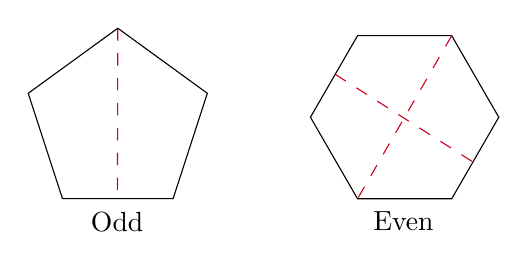
\begin{tikzpicture}[x=0.75pt,y=0.75pt,yscale=-1,xscale=1]
%uncomment if require: \path (0,300); %set diagram left start at 0, and has height of 300

%Straight Lines [id:da021745834724475888] 
\draw [color={rgb, 255:red, 208; green, 2; blue, 27 }  ,draw opacity=1 ] [dash pattern={on 4.5pt off 4.5pt}]  (93.18,37.75) -- (93,120) ;
%Shape: Regular Polygon [id:dp9055114382475318] 
\draw   (136.32,69.1) -- (119.84,119.82) -- (66.51,119.82) -- (50.03,69.1) -- (93.18,37.75) -- cycle ;
%Shape: Regular Polygon [id:dp98186031765677] 
\draw   (276.74,80.63) -- (254.06,119.92) -- (208.69,119.92) -- (186,80.63) -- (208.69,41.34) -- (254.06,41.34) -- cycle ;
%Straight Lines [id:da8263225516259709] 
\draw [color={rgb, 255:red, 208; green, 2; blue, 27 }  ,draw opacity=1 ] [dash pattern={on 4.5pt off 4.5pt}]  (254.06,41.34) -- (208.69,119.92) ;
%Straight Lines [id:da9512534405083728] 
\draw [color={rgb, 255:red, 208; green, 2; blue, 27 }  ,draw opacity=1 ] [dash pattern={on 4.5pt off 4.5pt}]  (198,60) -- (264,102) ;

% Text Node
\draw (79,125) node [anchor=north west][inner sep=0.75pt]   [align=left] {Odd};
% Text Node
\draw (215,125) node [anchor=north west][inner sep=0.75pt]   [align=left] {Even};


\end{tikzpicture}
\end{center}
When $n$ is odd, the $n$ reflections are in axis through the center and each of the vertices. For even $n$, we have $n/2$ reflections in axis through pairs of opposite vertices, and $n / 2$ reflections in axes through pairs of opposite midpoints of edges.

From this you should count $2n$ elements, and we will now see that there is no other elements.

\begin{proposition}
	A regular $n$-gon has $2n$ symmetries.
\end{proposition}
\begin{proof}
	Let $g \in D_{2n}$. Since $g$ is a symmetry of our $n$-gon, it must send vertices to vertices and edges to edges. So if $v_1$ is a vertex who's adjacent vertices are $v_2$ and $v_n$ and we have $g(v_1) = v_i$, then we must know $g(v_1)$ and $g(v_n)$, so we must know exactly what $g$. Since there is $n$ possibilities for where $v_1$ is sent, and $2$ possibilities for where $v_2$ is sent, there must be $2n$ elements in total.
\end{proof}

\begin{proposition}
	$D_{2n}$ is a group.
\end{proposition}
\begin{proof}
	We have closure by `composition of symmetries are also symmetries', identity with the `do nothing' symmetry and also inverses, as a rotation by $\frac{2 \pi k}{n}$ has an inverse of a $\frac{2\pi(n - k)}{n}$ rotation, and reflections are self inverse. We also have associativity, as the composition of functions is associative. Thus $D_{2n}$ is a group. 
\end{proof}

It's possible to generate every element in the group with just a single rotation and a reflection. Let $r$ be the rotation by $\frac{2\pi}{n}$, and let $s$ be the reflection about the axis through $v_1$ and the center. Then $r^k$ gives the rotation by $\frac{2 \pi k}{n}$ and we can perform any reflection by first rotating the $n$-gon, then applying the reflection, and then rotating back. 

$D_{2n}$ is also not abelian, and indeed we have $rs = sr^{-1}$.

\begin{aside}{Aside: Group Presentations}
One way to write groups is with a \vocab{presentation}. This is an expression of the form
$$
\langle \text{generators } \lvert \text{ relations between generators} \rangle.
$$
As an example, we can express the cyclic and dihedral groups using generators as follows
\begin{align*}
	C_n &= \langle a\mid  a^n = e \rangle \\
	D_{2n} &= \langle r, s \mid r^n = e,\; s^2 = e,\; rs = sr^{-1} \rangle
\end{align*}
You should be able to deduce all things that are true in the group from the relations in the presentation. However, you should be aware that there are some `caveats', for example if we wrote down
$$
\langle r, s \mid r^n = e, \; s^2 = e \rangle \neq D_{2n}.
$$
It is, in general, quite hard to write down a presentation for a given group, or even to determine the group from a given presentation. In this course, we will not look at the `mathematical tools' which allow us to discuss presentations in a rigerous 
way.

\begin{example}
	The group
	$$
	\left\langle a, b, c \mid a b a^{-1} b^{-1}=b, \; b c b^{-1} c^{-1}=c, \; cac^{-1} a^{-1}=a\right\rangle=\{e\},
	$$
	but the group
	$$
	\left\langle a, b, c, d \mid a b a^{-1} b^{-1}=b, \; b<b^{-1} c^{-1}=c,\; c d c^{-1} d^{1}=d, \; d a d^{-1} a^{1}=a\right\rangle
	$$
	is the \vocab{Higman group}, and it is infinite. It should be clear from this example that it is quite hard to determine a group from just it's presentation.
\end{example}

\end{aside}

\section{Permutation Groups}

We are now going to discuss groups made up of \emph{permutations}.

\begin{definition}[Permutations]
	Given a set $X$, a \vocab{permutation} of $X$ is a bijective function $\sigma: X \rightarrow X$. The set of all permutations of $X$ is denoted $\sym X$.
\end{definition}

\begin{theorem}
	For any set $X$, $\sym X$ is a group with respect to composition. 
\end{theorem}
\begin{proof}
	We check the group axioms individually.
	\begin{itemize}
		\item \emph{Closure}. The composition of two bijective functions from $X \rightarrow X$ is a bijective function from $X \rightarrow X$.
		\item \emph{Associativity}. Composition of functions is associative.
		\item \emph{Identity}. The identity function $\operatorname{id}(x) = x$ is bijective.
		\item \emph{Inverses}. Every bijective function has a bijective inverse.
	\end{itemize}
	Thus $\sym X$ is a group.
\end{proof}

\begin{definition}[Symmetric Group]
	If $|X| = n$, we write $S_n$ for (the isomorphism class of) $\sym X$. $S_n$ is the \vocab{symmetric group} on $n$ elements.
\end{definition}

It should be reasonably clear that $|S_n| = n(n - 1) \cdots 1 = n!$. We will also normally use $X = \{1, 2, 3, \dots, n \}$ when we study $S_n$. When dealing with permutation groups, it's helpful to have some notation to express permutations. For a general $\sigma \in S_n$, we write
$$
\sigma = \begin{pmatrix}
	1 & 2 & 3 & \cdots & n \\
	\sigma(1) & \sigma(2) & \sigma(3) & \cdots & \sigma(n)
\end{pmatrix}.
$$

\begin{example}
	If we had some $\sigma \in S_3$ such that $\sigma(1) = 2$, $\sigma(2) = 3$, and $\sigma(3) = 1$, we would write
	$$
\sigma = \begin{pmatrix}
	1 & 2 & 3 \\
	2 & 3 & 1
\end{pmatrix}.
$$
\end{example}

A slightly better notation for when we have a permutation that `cycles' some elements $a_1, \cdots a_k \in \{1, 2, \dots, n\}$ and leaves the other elements unchanged, we can write
$$
\sigma = \begin{pmatrix}
	a_1 & a_2 & \cdots & a_k
\end{pmatrix}
$$
which denotes the permutation mapping the elements as follows
\begin{center}
	

\tikzset{every picture/.style={line width=0.75pt}} %set default line width to 0.75pt        


\begin{tikzpicture}[x=0.75pt,y=0.75pt,yscale=-1,xscale=1]
%uncomment if require: \path (0,300); %set diagram left start at 0, and has height of 300

%Straight Lines [id:da564247942341451] 
\draw [color={rgb, 255:red, 208; green, 2; blue, 27 }  ,draw opacity=1 ]   (64.01,125) -- (97,125) ;
\draw [shift={(100,125)}, rotate = 180] [fill={rgb, 255:red, 208; green, 2; blue, 27 }  ,fill opacity=1 ][line width=0.08]  [draw opacity=0] (8.93,-4.29) -- (0,0) -- (8.93,4.29) -- cycle    ;
%Straight Lines [id:da729246940968933] 
\draw [color={rgb, 255:red, 208; green, 2; blue, 27 }  ,draw opacity=1 ]   (120.33,125) -- (153.32,125) ;
\draw [shift={(156.32,125)}, rotate = 180] [fill={rgb, 255:red, 208; green, 2; blue, 27 }  ,fill opacity=1 ][line width=0.08]  [draw opacity=0] (8.93,-4.29) -- (0,0) -- (8.93,4.29) -- cycle    ;
%Straight Lines [id:da8820978230555316] 
\draw [color={rgb, 255:red, 208; green, 2; blue, 27 }  ,draw opacity=1 ]   (176.89,125) -- (209.87,125) ;
\draw [shift={(212.87,125)}, rotate = 180] [fill={rgb, 255:red, 208; green, 2; blue, 27 }  ,fill opacity=1 ][line width=0.08]  [draw opacity=0] (8.93,-4.29) -- (0,0) -- (8.93,4.29) -- cycle    ;
%Straight Lines [id:da5006305027432474] 
\draw [color={rgb, 255:red, 208; green, 2; blue, 27 }  ,draw opacity=1 ]   (246.44,125) -- (279.43,125) ;
\draw [shift={(282.43,125)}, rotate = 180] [fill={rgb, 255:red, 208; green, 2; blue, 27 }  ,fill opacity=1 ][line width=0.08]  [draw opacity=0] (8.93,-4.29) -- (0,0) -- (8.93,4.29) -- cycle    ;
%Curve Lines [id:da45854715793721934] 
\draw [color={rgb, 255:red, 208; green, 2; blue, 27 }  ,draw opacity=1 ]   (310.51,126) .. controls (406.52,168.45) and (-77.12,171.97) .. (38.06,124.72) ;
\draw [shift={(39.84,124)}, rotate = 518.5] [fill={rgb, 255:red, 208; green, 2; blue, 27 }  ,fill opacity=1 ][line width=0.08]  [draw opacity=0] (8.93,-4.29) -- (0,0) -- (8.93,4.29) -- cycle    ;

% Text Node
\draw (45.77,117.4) node [anchor=north west][inner sep=0.75pt]    {$a_{1}$};
% Text Node
\draw (101.81,117.4) node [anchor=north west][inner sep=0.75pt]    {$a_{2}$};
% Text Node
\draw (158.36,117.4) node [anchor=north west][inner sep=0.75pt]    {$a_{3}$};
% Text Node
\draw (218.86,120.4) node [anchor=north west][inner sep=0.75pt]    {$\cdots $};
% Text Node
\draw (289.47,117.4) node [anchor=north west][inner sep=0.75pt]    {$a_{k}$};


\end{tikzpicture}

\end{center}
The cyclic nature of this notation also implies that the two permutations $(a_1\; a_2\; \cdots\; a_k) = (a_2\; a_3\; \cdots\; a_k\; a_1)$. To define this notation slightly more formally, we have
$$
\begin{pmatrix}
	a_1 & a_2 & \cdots & a_k
\end{pmatrix} (x) = \begin{cases}
	a_{i + 1} &\mbox{if } x = a_i, \; (i < k) \\
	a_1 &\mbox{if } x = a_k \\
	x &\mbox{if } x \not \in \{a_1, a_2, \dots, a_k\}.
   \end{cases}
$$
We distinguish between permutations that can be written directly in this form in the following way.
\begin{definition}[Cycles and Transpositions]
	A permutation of the form $\sigma = (a_1\; a_2\; \cdots\; a_k)$ is a \vocab{$k$-cycle}. If $k = 2$ then we call it a \vocab{transposition}.
\end{definition}

As cycles are permutations, we can compose them.
\begin{example}[Composing Cycles]
If we consider the composition of two cycles $(1\; 2\; 3\; 4)(3 \; 2\; 4)$, this should be a permutation in $S_4$. Indeed we have
\begin{align*}
	1 &\longmapsto 1 \longmapsto 2 \\
	2 &\longmapsto 4 \longmapsto 1 \\
	3 &\longmapsto 2 \longmapsto 3 \\
	4 &\longmapsto 3 \longmapsto 4 \\
\end{align*}
So we actually have that the composition of these cycles is also a cycle\footnote{This is, in general, not the case}, namely $(1\; 2\; 3\; 4)(3 \; 2\; 4) = (1\; 2)$. 
\end{example}

In the example above, the two cycles involved elements that were in both cycles. We have a specific term for when this is not the case.

\begin{definition}[Disjoint Cycles]
	We say that two cycles are \vocab{disjoint} if no number appears in both cycles.
\end{definition}
\begin{lemma}
	Disjoint cycles commute.
\end{lemma}
\begin{proof}
	Let $\sigma, \tau \in S_n$ be two disjoint cycles. We want to show that $\sigma \tau = \tau \sigma$, that is, for any $x \in \{1, 2, \dots, n\}$, we have $\sigma(\tau(x)) = \tau(\sigma(x))$. We have two cases.

	If $x$ is in neither $\sigma$ or $\tau$, then $\sigma(x) = \tau(x) = x$, and thus $\sigma(\tau(x)) = \tau(\sigma(x)) = x$.

	Otherwise $x$ is in exactly one of $\sigma$ or $\tau$. WLOG let it be in $\sigma$. Then $\sigma(x)$ is also in $\sigma$ (and hence not $\tau$), so $\tau(x) = x$ and $\tau(\sigma(x)) = \sigma(x)$. Thus $\sigma(\tau(x)) = \sigma(x)$, so they commute.
\end{proof}

Slightly more suprising is the following theorem
\begin{theorem}[Writing Permutations with Cycles]
	Any $\sigma \in S_n$ can be written uniquely\footnote{Up to the order of the cycles in the composition} as the composition of disjoint cycles.
\end{theorem}
\begin{proof}
	First we show that any permutation can be written as the composition of cycles.
	Take $\sigma \in S_n$, and consider $1, \sigma(1), \sigma^2(1), \dots$. Since $\{1, 2, \dots, n\}$ is finite, there must exist $a > b$ such that $\sigma^a(1) = \sigma^b(1)$. So $\sigma^{a -b}(1) = 1$. Now let $k > 0$ be the smallest integer such that $\sigma^k(1) = 1$, which must exist by the previous argument. Then for $0 \leq l < m < k$, if $\sigma^m(1) = \sigma^l(1)$, then $\sigma^{m - l}(1) = 1$, which contradicts the minimality of $k$. So all of $1, \sigma(1), \sigma^2(1), \dots, \sigma^k(1)$ are distinct. This gives us our first cycle $(1\; \sigma(1)\; \sigma^2(1)\; \sigma^{k - 1}(1))$.
	We can repeat this process for the next number in $\{1, 2, \dots, n\}$ that has not already appeared, until eventually every element has appeared. As $\sigma$ is a bijection, no element can reappear.

	We now show that this composition of cycles is unique up to the order of composition. Suppose we have two such decompositions
	\begin{align*}
		\sigma &= (a_1 \; \cdots \; a_{k_1}) (a_{k_{1 + i}} \; \cdots \; a_{k_2}) \cdots (a_{k_{m - 1}} \; \cdots \; a_{k_m})\\
		  &= (b_1 \; \cdots \; b_{k_1}) (b_{k_{1 + i}} \; \cdots \; b_{k_2}) \cdots (b_{k_{m - 1}} \; \cdots \; b_{k_m})
	\end{align*}
	and each $j \in \{1, 2, \dots, n\}$ appears exactly once in both. Then we have $a_1 = b_t$ for some $t$, and the other numbers in the cycle are uniquely determined by $\sigma(a_1), \sigma^2(a_1), \dots$. So we have
	$$
	(a_1\; \cdots\; a_{k_1}) (\cdots) = (b_t\; \cdots)(\cdots),
	$$
	since disjoint cycles commute and we can `cycle' the elements in cycles. If we continue this, we will find that all other cycles match too.
\end{proof}

\clearpage
\chapter*{Biblography}

TODO: Make this proper.

\begin{itemize}
	\item Napkin by Evan Chen -- Used for a good few of the examples
	\item Abstract Algebra by Dummit and Foote -- General Reference
	\item A Book of Abstract Algebra, Charles Pinter -- General Reference
	\item Dexter Chua and David Bai's notes -- For a general view on the course structure before the lectures were completed, along with some of the proofs that were omitted from our lectures.
\end{itemize}

\end{document}
